\documentclass[tikz,border=2pt]{standalone}
\usepackage{amsmath,amssymb}
\usepackage{pgfplots}
\pgfplotsset{compat=1.18}
\usetikzlibrary{arrows.meta}
\begin{document}
% Barber's shop (Exercise 5.2.7): M/M/1/K with lambda = 6, mu = 5, rho = 1.2; p(n) = rho^n / sum_{j<=K} rho^j.
% Left K = 3: (0.186, 0.224, 0.268, 0.322); right K = 6: (0.077, 0.093, 0.112, 0.134, 0.161, 0.193, 0.231).
% The bar at n = K (orange) is the blocking probability p(K) = pi(K).
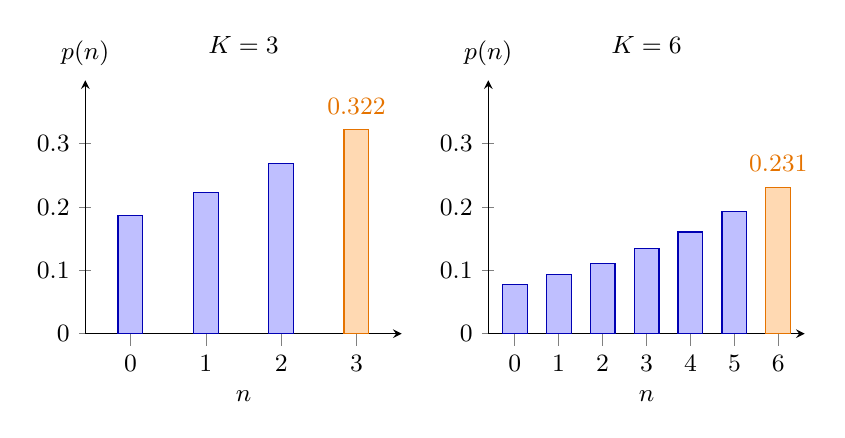
\begin{tikzpicture}[font=\small, >={Latex[length=2mm]}]
  \pgfplotsset{barstyle/.style={
    axis lines=left, ymin=0, ymax=0.4, ytick={0,0.1,0.2,0.3},
    yticklabel style={/pgf/number format/fixed, /pgf/number format/precision=1},
    ybar, bar width=9pt, bar shift=0pt, xlabel={$n$}, width=5.6cm, height=4.8cm, clip=false,
    ylabel style={rotate=-90, anchor=south, at={(axis description cs:0,1.02)}}}}
  \begin{axis}[barstyle, name=left, xmin=-0.6, xmax=3.6, xtick={0,1,2,3}, ylabel={$p(n)$}, title={$K=3$}]
    \addplot[draw=blue!70!black, fill=blue!25] coordinates {(0,0.1863) (1,0.2235) (2,0.2683)};
    \addplot[draw=orange!90!black, fill=orange!30] coordinates {(3,0.3219)};
    \node[orange!90!black, anchor=south] at (axis cs:3,0.33) {$0.322$};
  \end{axis}
  \begin{axis}[barstyle, at={(left.east)}, anchor=west, xshift=1.1cm, xmin=-0.6, xmax=6.6, xtick={0,...,6}, ylabel={$p(n)$}, title={$K=6$}]
    \addplot[draw=blue!70!black, fill=blue!25] coordinates {(0,0.0774) (1,0.0929) (2,0.1115) (3,0.1338) (4,0.1605) (5,0.1927)};
    \addplot[draw=orange!90!black, fill=orange!30] coordinates {(6,0.2312)};
    \node[orange!90!black, anchor=south] at (axis cs:6,0.24) {$0.231$};
  \end{axis}
\end{tikzpicture}
\end{document}
